% !TEX program = pdflatex
\documentclass[10pt, aspectratio=169]{beamer}

% ── Theme & Colours ──────────────────────────────────────────────────
\usetheme{Madrid}
\usecolortheme{seahorse}
\setbeamertemplate{navigation symbols}{}
\setbeamertemplate{footline}[frame number]

% ── Packages ─────────────────────────────────────────────────────────
\usepackage{amsmath, amssymb, bm}
\usepackage{graphicx}
\usepackage{booktabs}
\usepackage{tikz}
\usetikzlibrary{arrows.meta, positioning, calc}
\usepackage{algorithm2e}
\usepackage{hyperref}
\usepackage{xcolor}

% ── Custom commands ──────────────────────────────────────────────────
\newcommand{\R}{\mathbb{R}}
\newcommand{\E}{\mathbb{E}}
\newcommand{\Var}{\operatorname{Var}}
\newcommand{\Cov}{\operatorname{Cov}}
\DeclareMathOperator*{\argmin}{arg\,min}

% ── Title ────────────────────────────────────────────────────────────
\title[Dynamic-PCI Pairs Trading]{%
  Dynamic Partial Cointegration for Pairs Trading\\[4pt]
  \large Kalman Filter--Based Hedge Ratio Tracking \& Spread Decomposition}
\author{Aryan Deo}
\institute{Undergraduate Project (UGP)}
\date{\today}

% =====================================================================
\begin{document}

% ─────────────────────────────────────────────────────────────────────
\begin{frame}
  \titlepage
\end{frame}

% ─────────────────────────────────────────────────────────────────────
\begin{frame}{Outline}
  \tableofcontents
\end{frame}

% =====================================================================
\section{Introduction \& Motivation}
% =====================================================================

\begin{frame}{Pairs Trading --- The Big Picture}
  \begin{itemize}
    \item \textbf{Pairs trading} exploits temporary mispricings between two
          co-moving assets.
    \item Classical approach: find cointegrated pairs during a
          \emph{formation period}, trade the spread during a subsequent
          \emph{trading period}.
    \item \textbf{Two key limitations} of the classical framework:
    \begin{enumerate}
      \item The hedge ratio $\beta$ is estimated \emph{once} (OLS) and held
            fixed --- but the true economic relationship drifts over time.
      \item The spread $X_{2,t} - \beta X_{1,t}$ is assumed \emph{fully
            stationary} --- but in reality part of the spread may be a
            permanent (random-walk) component.
    \end{enumerate}
    \item \textbf{Our contribution:} a \emph{Dynamic Partial Cointegration}
          (Dynamic-PCI) model that addresses both issues simultaneously
          using a Kalman filter.
  \end{itemize}
\end{frame}

% ─────────────────────────────────────────────────────────────────────
\begin{frame}{Literature Foundation}
  Our model unifies two strands of the literature:
  \vspace{6pt}
  \begin{columns}[T]
    \begin{column}{0.48\textwidth}
      \textbf{Yu (2023)}\\[3pt]
      \emph{``Cointegration Approach for Pair Trading Based on the
      Kalman Filter''}
      \begin{itemize}
        \item Models the hedge ratio $\beta_t$ as a \textbf{random walk},
              tracked in real time by a Kalman filter.
        \item Allows the hedging relationship to adapt to structural shifts.
      \end{itemize}
    \end{column}
    \begin{column}{0.48\textwidth}
      \textbf{Clegg \& Krauss (2018)}\\[3pt]
      \emph{``Pairs Trading with Partial Cointegration''}
      \begin{itemize}
        \item Decomposes the spread into a \textbf{mean-reverting} (AR(1))
              component $M_t$ and a \textbf{random-walk} component $R_t$.
        \item Only $M_t$ is tradeable; $R_t$ captures permanent shocks.
        \item Introduces $R^2_{\text{MR}}$ to measure the
              ``degree of cointegration.''
      \end{itemize}
    \end{column}
  \end{columns}
  \vspace{8pt}
  \begin{block}{Dynamic-PCI = Yu's dynamic $\beta_t$ + Clegg \& Krauss's $(X_{1,t}, M_t, R_t)$ state system}
    Joint 4-state vector $\bm{z}_t = [X_{1,t},\; \beta_t,\; M_t,\; R_t]^\top$ estimated
    in a unified Kalman filter framework with $4 \times 4$ transition matrix $\bm{F}$.
  \end{block}
\end{frame}

% =====================================================================
\section{The Dynamic-PCI Model}
% =====================================================================

\begin{frame}{Model Specification --- Observation Equation}
  \begin{block}{Observation (Measurement) System}
    \vspace{-4pt}
    \begin{align}
      X_{2,t} &= \underbrace{\beta_t \cdot X_{1,t}}_{\text{hedged component}}
               \;+\; \underbrace{M_t}_{\substack{\text{mean-reverting}\\\text{(tradeable)}}}
               \;+\; \underbrace{R_t}_{\substack{\text{random walk}\\\text{(permanent)}}}
               \label{eq:obs_x2}\\[4pt]
      X_{1,t} &= X_{1,t} \label{eq:obs_x1}
    \end{align}
  \end{block}
  \vspace{3pt}
  \begin{itemize}
    \item $X_{1,t}, X_{2,t}$: daily adjusted close prices of Asset~1 and Asset~2.
    \item Equation~\eqref{eq:obs_x2} models the spread relation between $X_2$ and $X_1$
          with a \textbf{time-varying hedge ratio} $\beta_t$.
    \item Equation~\eqref{eq:obs_x1} retains the driver asset in the observation vector
          $\bm{y}_t = \begin{bmatrix} X_{2,t} & X_{1,t} \end{bmatrix}^\top$, preserving the
          structural relation of static PCI (Clegg \& Krauss, 2018).
    \item $M_t$: \emph{transient mispricing} that reverts to zero --- what we trade.
    \item $R_t$: accumulated permanent shocks --- what we must \emph{not} trade.
  \end{itemize}
\end{frame}

% ─────────────────────────────────────────────────────────────────────
\begin{frame}{Model Specification --- State Equations ($4$ States)}
  \begin{block}{State Transition (Process) Equations}
    \vspace{-2pt}
    \begin{align}
      X_{1,t} &= X_{1,t-1} + w_t^{(X)},
        &w_t^{(X)} &\sim \mathcal{N}(0,\; \sigma_X^2)
        \quad \text{\small(Driver asset random walk; Clegg \& Krauss)}
        \label{eq:X1}\\[3pt]
      \beta_t &= \beta_{t-1} + w_t^{(\beta)},
        &w_t^{(\beta)} &\sim \mathcal{N}(0,\; q_\beta)
        \quad \text{\small(Dynamic hedge ratio random walk; Yu)}
        \label{eq:beta}\\[3pt]
      M_t &= \rho\, M_{t-1} + w_t^{(M)},
        &w_t^{(M)} &\sim \mathcal{N}(0,\; \sigma_M^2)
        \quad \text{\small(Mean-reverting transient spread)}
        \label{eq:M}\\[3pt]
      R_t &= R_{t-1} + w_t^{(R)},
        &w_t^{(R)} &\sim \mathcal{N}(0,\; \sigma_R^2)
        \quad \text{\small(Random-walk permanent drift)}
        \label{eq:R}
    \end{align}
  \end{block}
  \vspace{2pt}
  \begin{itemize}
    \item $|\rho| < 1$ guarantees $M_t$ mean-reverts with half-life $h = \dfrac{\ln 0.5}{\ln \rho}$ days.
    \item Retaining $X_{1,t}$ preserves the fundamental price dynamics of Asset~1 from static PCI.
    \item $q_\beta = 0$ locks $\beta_t \equiv \beta$, recovering the \textbf{static-PCI} model as a special case.
    \item All innovations $w_t^{(X)}, w_t^{(\beta)}, w_t^{(M)}, w_t^{(R)}$ are mutually independent.
  \end{itemize}
\end{frame}

% ─────────────────────────────────────────────────────────────────────
\begin{frame}{Compact State-Space Representation ($4 \times 4$ System)}
  Define the full state vector
  $\bm{z}_t = \begin{bmatrix}X_{1,t} & \beta_t & M_t & R_t\end{bmatrix}^\top \in \mathbb{R}^4$.
  \vspace{4pt}
  \begin{block}{State Equation ($4 \times 4$ Transition Matrix $\bm{F}$)}
    \[
      \bm{z}_t = \bm{F}\,\bm{z}_{t-1} + \bm{w}_t,\qquad
      \bm{F} = \begin{bmatrix}
        1 & 0 & 0 & 0\\
        0 & 1 & 0 & 0\\
        0 & 0 & \rho & 0\\
        0 & 0 & 0 & 1
      \end{bmatrix},\qquad
      \bm{Q} = \begin{bmatrix}
        \sigma_X^2 & 0 & 0 & 0\\
        0 & q_\beta & 0 & 0\\
        0 & 0 & \sigma_M^2 & 0\\
        0 & 0 & 0 & \sigma_R^2
      \end{bmatrix}
    \]
  \end{block}
  \begin{block}{Observation Equation (Coupling $X_2$ and $X_1$)}
    \[
      \bm{y}_t = \begin{bmatrix} X_{2,t} \\ X_{1,t} \end{bmatrix} = \bm{H}_t\,\bm{z}_t,\qquad
      \bm{H}_t = \begin{bmatrix}
        0 & X_{1,t} & 1 & 1\\[2pt]
        1 & 0 & 0 & 0
      \end{bmatrix}
    \]
  \end{block}
  \vspace{2pt}
  \begin{itemize}
    \item Row~1 gives $X_{2,t} = X_{1,t}\,\beta_t + M_t + R_t$ (pairs spread relationship).
    \item Row~2 gives $X_{1,t} = X_{1,t}$ (observes driver asset price directly).
    \item Notice: $\bm{F}$ is \textbf{$4 \times 4$}, unifying Clegg \& Krauss's 3-state system with Yu's dynamic $\beta_t$.
  \end{itemize}
\end{frame}

% ─────────────────────────────────────────────────────────────────────
\begin{frame}{State-Space Comparison: Static-PCI vs.\ Dynamic-PCI}
  \begin{columns}[T]
    \begin{column}{0.48\textwidth}
      \textbf{Static-PCI (Clegg \& Krauss, 2018)}
      \begin{itemize}
        \item State: $\bm{z}_t^{\text{stat}} = \begin{bmatrix}X_{1,t} & M_t & R_t\end{bmatrix}^\top$ ($3 \times 1$)
        \item Hedge ratio $\beta$ is a \textbf{constant parameter} estimated via MLE (outside state).
        \item Transition matrix ($3 \times 3$):
          \[
            \bm{F}_{\text{stat}} = \begin{bmatrix}1 & 0 & 0\\ 0 & \rho & 0\\ 0 & 0 & 1\end{bmatrix}
          \]
        \item Observation matrix ($2 \times 3$):
          \[
            \bm{H}_{\text{stat}} = \begin{bmatrix}\beta & 1 & 1\\ 1 & 0 & 0\end{bmatrix}
          \]
      \end{itemize}
    \end{column}
    \begin{column}{0.48\textwidth}
      \textbf{Dynamic-PCI (Our Proposed Model)}
      \begin{itemize}
        \item State: $\bm{z}_t = \begin{bmatrix}X_{1,t} & \beta_t & M_t & R_t\end{bmatrix}^\top$ (\textbf{$4 \times 1$})
        \item Hedge ratio $\beta_t$ is a \textbf{dynamic state} driven by random-walk noise $q_\beta$.
        \item Transition matrix (\textbf{$4 \times 4$}):
          \[
            \bm{F} = \begin{bmatrix}1 & 0 & 0 & 0\\ 0 & 1 & 0 & 0\\ 0 & 0 & \rho & 0\\ 0 & 0 & 0 & 1\end{bmatrix}
          \]
        \item Observation matrix ($2 \times 4$):
          \[
            \bm{H}_t = \begin{bmatrix}0 & X_{1,t} & 1 & 1\\ 1 & 0 & 0 & 0\end{bmatrix}
          \]
      \end{itemize}
    \end{column}
  \end{columns}
  \vspace{6pt}
  \begin{block}{Theoretical Equivalence at $q_\beta = 0$}
    When $q_\beta = 0$, $\beta_t \equiv \beta$, and column 2 of $\bm{H}_t$ contracts into column 1,
    recovering Clegg \& Krauss's exact observation matrix $\begin{bmatrix}\beta & 1 & 1\\ 1 & 0 & 0\end{bmatrix}$.
  \end{block}
\end{frame}

% ─────────────────────────────────────────────────────────────────────
\begin{frame}{Key Derived Quantities}
  \begin{columns}[T]
    \begin{column}{0.50\textwidth}
      \textbf{Mean-Reversion Ratio} (Clegg \& Krauss)
      \[
        R^2_{\text{MR}} = \frac{2\,\sigma_M^2}{2\,\sigma_M^2 + (1+\rho)\,\sigma_R^2}
      \]
      \begin{itemize}
        \item $R^2_{\text{MR}} \to 1$: spread is mostly mean-reverting
              $\Rightarrow$ highly tradeable.
        \item $R^2_{\text{MR}} \to 0$: spread is mostly a random walk
              $\Rightarrow$ not suitable for pairs trading.
      \end{itemize}
    \end{column}
    \begin{column}{0.45\textwidth}
      \textbf{Half-Life of Mean Reversion}
      \[
        h = \frac{\ln(0.5)}{\ln(\rho)} \quad \text{(days)}
      \]
      \begin{itemize}
        \item Determines how quickly a mispricing is expected to close.
        \item Directly informs position holding period and risk management.
      \end{itemize}
    \end{column}
  \end{columns}
\end{frame}

% =====================================================================
\section{Kalman Filter Derivation}
% =====================================================================

\begin{frame}{Kalman Filter --- Predict Step ($4 \times 4$ System)}
  At each time step $t$, given posterior $(\hat{\bm{z}}_{t-1|t-1},\; \bm{P}_{t-1|t-1})$:
  \vspace{6pt}
  \begin{block}{Prediction (Time Update)}
    \begin{align}
      \hat{\bm{z}}_{t|t-1} &= \bm{F}\,\hat{\bm{z}}_{t-1|t-1}
        \label{eq:predict_z}\\[6pt]
      \bm{P}_{t|t-1} &= \bm{F}\,\bm{P}_{t-1|t-1}\,\bm{F}^\top + \bm{Q}
        \label{eq:predict_P}
    \end{align}
  \end{block}
  \vspace{4pt}
  Expanding element-wise for each of the $4$ states:
  \[
    \hat{X}_{1,t|t-1} = \hat{X}_{1,t-1|t-1},\qquad
    \hat{\beta}_{t|t-1} = \hat{\beta}_{t-1|t-1},\qquad
    \hat{M}_{t|t-1} = \rho\,\hat{M}_{t-1|t-1},\qquad
    \hat{R}_{t|t-1} = \hat{R}_{t-1|t-1}
  \]
  \vspace{2pt}
  \begin{itemize}
    \item $\hat{X}_{1,t|t-1}$ and $\hat{R}_{t|t-1}$ propagate as martingales (unit roots).
    \item $\hat{\beta}_{t|t-1}$ persists at previous filtered estimate (random walk).
    \item $\hat{M}_{t|t-1}$ contracts toward zero by a factor of $\rho$ (mean reversion).
  \end{itemize}
\end{frame}

% ─────────────────────────────────────────────────────────────────────
\begin{frame}{Kalman Filter --- Update Step}
  Given observation vector $\bm{y}_t = \begin{bmatrix}X_{2,t} & X_{1,t}\end{bmatrix}^\top$:
  \vspace{3pt}
  \begin{block}{Measurement Update}
    \begin{align}
      \text{Innovation ($2 \times 1$):}\quad \bm{e}_t &= \bm{y}_t - \bm{H}_t\,\hat{\bm{z}}_{t|t-1}
        = \begin{bmatrix} X_{2,t} - (X_{1,t}\,\hat{\beta}_{t|t-1} + \hat{M}_{t|t-1} + \hat{R}_{t|t-1}) \\
                          X_{1,t} - \hat{X}_{1,t|t-1} \end{bmatrix}
        \label{eq:innov}\\[3pt]
      \text{Innovation variance ($2 \times 2$):}\quad \bm{S}_t &= \bm{H}_t\,\bm{P}_{t|t-1}\,\bm{H}_t^\top
        \label{eq:innov_var}\\[3pt]
      \text{Kalman gain ($4 \times 2$):}\quad \bm{K}_t &= \bm{P}_{t|t-1}\,\bm{H}_t^\top\,\bm{S}_t^{-1}
        \label{eq:gain}\\[3pt]
      \text{State update ($4 \times 1$):}\quad \hat{\bm{z}}_{t|t} &= \hat{\bm{z}}_{t|t-1} + \bm{K}_t\,\bm{e}_t
        \label{eq:update_z}\\[3pt]
      \text{Covariance update ($4 \times 4$):}\quad \bm{P}_{t|t} &= (\bm{I}_4 - \bm{K}_t\,\bm{H}_t)\,\bm{P}_{t|t-1}
        \label{eq:update_P}
    \end{align}
  \end{block}
  \vspace{2pt}
  \begin{itemize}
    \item \textbf{Exact Driver Price Condition:} Because $X_{1,t}$ is observed without measurement noise,
          conditioning on $X_{1,t}$ sets $\hat{X}_{1,t|t} \equiv X_{1,t}$. The remaining states $(\beta_t, M_t, R_t)$
          are simultaneously updated by the scalar spread innovation $e_{1,t} = X_{2,t} - \hat{X}_{2,t|t-1}$.
  \end{itemize}
\end{frame}

% ─────────────────────────────────────────────────────────────────────
\begin{frame}{Kalman Filter --- Initialization ($4 \times 4$ System)}
  \begin{block}{Initial Conditions ($t = 0$)}
    \[
      \hat{\bm{z}}_{0|0} = \begin{bmatrix}X_{1,0}\\[2pt] \beta_0\\[2pt] 0\\[2pt] X_{2,0} - \beta_0\,X_{1,0}\end{bmatrix},\qquad
      \bm{P}_{0|0} = \begin{bmatrix}
        \epsilon_X & 0 & 0 & 0\\
        0 & p_{\beta_0} & 0 & 0\\
        0 & 0 & \epsilon & 0\\
        0 & 0 & 0 & \epsilon
      \end{bmatrix}
    \]
  \end{block}
  \vspace{4pt}
  \begin{itemize}
    \item $X_{1,0}$: initialized to the observed Asset~1 price ($\epsilon_X = 10^{-8}$).
    \item $\beta_0$: initial hedge-ratio estimate (from MLE formation fit).
    \item $M_0 = 0$: assume no initial mispricing ($\epsilon = 10^{-8}$).
    \item $R_0 = X_{2,0} - \beta_0 X_{1,0}$: residual assigned initially to permanent drift.
    \item $p_{\beta_0} = 1.0$: reflects initial prior uncertainty in hedge ratio $\beta$.
  \end{itemize}
\end{frame}

% =====================================================================
\section{Parameter Estimation: Maximum Likelihood}
% =====================================================================

\begin{frame}{Prediction Error Decomposition}
  The Partial Cointegration model parameters $\bm{\theta} = (\beta_0,\;\rho,\;\sigma_M,\;\sigma_R,\;q_\beta)$
  are estimated by \textbf{maximum likelihood} on formation data:
  \begin{block}{Log-Likelihood (Durbin \& Koopman, 2012)}
    \[
      \ell(\bm{\theta}) = -\frac{1}{2}\sum_{t=1}^{T_{\text{form}}}
        \left[\ln(2\pi\,S_t) + \frac{e_t^2}{S_t}\right]
    \]
  \end{block}
  where $e_t$ and $S_t$ are the spread innovation and its variance from the 4-state Kalman filter.
  \vspace{4pt}
  \begin{itemize}
    \item \textbf{Optimization:} L-BFGS-B over $(\beta_0,\; \rho,\; \ln\sigma_M,\; \ln\sigma_R,\; \ln q_\beta)$.
    \item \textbf{Model comparison:} Likelihood-ratio test vs.\ static baseline
          ($q_\beta = 10^{-12}$).
  \end{itemize}
\end{frame}

% =====================================================================
\section{Data Pipeline}
% =====================================================================

\begin{frame}{Data Pipeline Overview}
  \begin{center}
  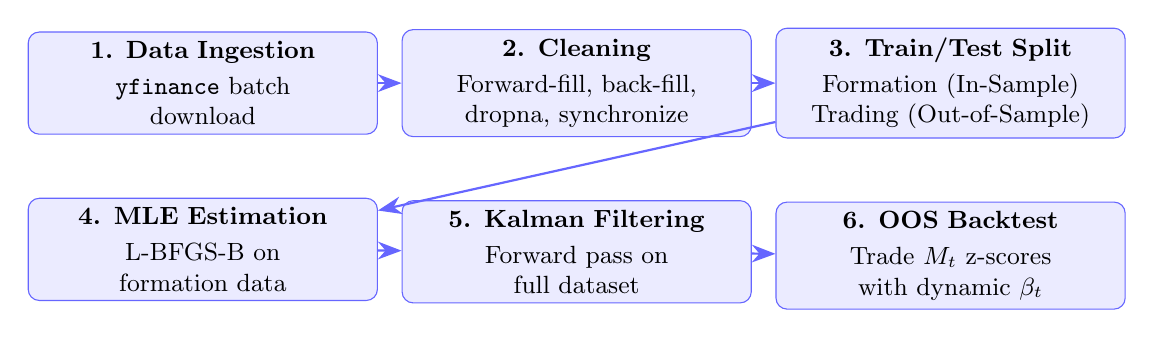
\begin{tikzpicture}[
    node distance=0.8cm and 0.3cm,
    block/.style={rectangle, draw=blue!60, fill=blue!8, rounded corners,
                  text width=4.2cm, minimum height=1cm, align=center, font=\small},
    arrow/.style={-{Stealth[length=3mm]}, thick, blue!60},
  ]
    \node[block] (A) {\textbf{1. Data Ingestion}\\[2pt]\texttt{yfinance} batch\\download};
    \node[block, right=of A] (B) {\textbf{2. Cleaning}\\[2pt]Forward-fill, back-fill,\\dropna, synchronize};
    \node[block, right=of B] (C) {\textbf{3. Train/Test Split}\\[2pt]Formation (In-Sample)\\Trading (Out-of-Sample)};
    \node[block, below=of A] (D) {\textbf{4. MLE Estimation}\\[2pt]L-BFGS-B on\\formation data};
    \node[block, below=of B] (E) {\textbf{5. Kalman Filtering}\\[2pt]Forward pass on\\full dataset};
    \node[block, below=of C] (F) {\textbf{6. OOS Backtest}\\[2pt]Trade $M_t$ z-scores\\with dynamic $\beta_t$};
    \draw[arrow] (A) -- (B);
    \draw[arrow] (B) -- (C);
    \draw[arrow] (C) -- (D);
    \draw[arrow] (D) -- (E);
    \draw[arrow] (E) -- (F);
  \end{tikzpicture}
  \end{center}
\end{frame}

% ─────────────────────────────────────────────────────────────────────
\begin{frame}{Data Specification}
  \begin{columns}[T]
    \begin{column}{0.48\textwidth}
      \textbf{Target Pairs (7 pairs)}
      \vspace{4pt}
      \begin{table}[h]
        \centering\small
        \begin{tabular}{@{}ll@{}}
          \toprule
          Asset 1 ($X_1$) & Asset 2 ($X_2$) \\
          \midrule
          AAP  & IBM \\
          EWA  & EWC \\
          NKE  & AES \\
          MRK  & VZ  \\
          GS   & CVX \\
          KO   & PEP \\
          XOM  & CVX \\
          \bottomrule
        \end{tabular}
      \end{table}
    \end{column}
    \begin{column}{0.48\textwidth}
      \textbf{Date Ranges}
      \vspace{4pt}
      \begin{itemize}
        \item \textbf{Formation (In-Sample):}\\
              2009-09-01 to 2013-08-31\\
              ($\approx$ 4 years, $\sim$1000 trading days)
        \item \textbf{Trading (Out-of-Sample):}\\
              2013-09-01 to 2021-08-31\\
              ($\approx$ 8 years, $\sim$2000 trading days)
        \item \textbf{Source:} Yahoo Finance daily adjusted close prices.
        \item \textbf{Cleaning:} Forward-fill $\to$ back-fill $\to$ dropna
              to achieve 100\% synchronous timestamps.
      \end{itemize}
    \end{column}
  \end{columns}
\end{frame}

% =====================================================================
\section{Trading Strategy \& Backtesting}
% =====================================================================

\begin{frame}{Signal Construction}
  \begin{block}{Core Idea (Clegg \& Krauss)}
    Trade the \textbf{z-score of $M_t$}, not the raw spread
    $X_{2,t} - \beta_t X_{1,t}$.
  \end{block}
  \vspace{4pt}

  \textbf{Z-score computation} (expanding window):
  \[
    z_t = \frac{M_t - \bar{M}_{1:t}}{\hat{\sigma}_{M,\,1:t}}
  \]
  where $\bar{M}_{1:t}$ and $\hat{\sigma}_{M,\,1:t}$ are the expanding
  mean and standard deviation of $M$ up to time $t$.

  \vspace{6pt}
  \textbf{Entry/exit rules:}
  \begin{itemize}
    \item \textbf{Open long spread} ($+1$) when $z_t < -\tau_{\text{open}}$
          (spread too low, expect reversion up).
    \item \textbf{Open short spread} ($-1$) when $z_t > +\tau_{\text{open}}$
          (spread too high, expect reversion down).
    \item \textbf{Close position} when $z_t$ crosses $\mp\tau_{\text{close}}$
          (spread has reverted sufficiently).
    \item Default: $\tau_{\text{open}} = 1.0$, $\tau_{\text{close}} = 0.5$.
  \end{itemize}
\end{frame}

% ─────────────────────────────────────────────────────────────────────
\begin{frame}{Position Sizing \& P\&L}
  \textbf{Hedge-ratio-weighted pair portfolio:}
  \begin{itemize}
    \item Long spread ($+1$): \emph{long} 1 unit of $X_2$, \emph{short}
          $\beta_t$ units of $X_1$.
    \item Short spread ($-1$): reverse.
    \item The hedge ratio $\beta_t$ \textbf{adapts daily} via the Kalman filter
          (the Yu contribution).
  \end{itemize}

  \vspace{6pt}
  \textbf{Daily P\&L} (normalized by notional):
  \[
    r_t^{\text{pair}} = \text{pos}_{t-1}\left(
      \frac{1}{1+|\beta_{t-1}|}\cdot r_t^{(X_2)}
      - \frac{\beta_{t-1}}{1+|\beta_{t-1}|}\cdot r_t^{(X_1)}
    \right)
  \]
  where $r_t^{(X_i)} = X_{i,t}/X_{i,t-1} - 1$.

  \vspace{6pt}
  \textbf{Transaction costs:} 5~bps ($0.0005$) per half-turn on each leg,
  applied on every position change (matching Clegg \& Krauss).
\end{frame}

% ─────────────────────────────────────────────────────────────────────
\begin{frame}{Performance Metrics}
  \begin{itemize}
    \item \textbf{Cumulative equity:}
      $\text{Equity}_t = \prod_{s=1}^{t}(1 + r_s^{\text{pair}})$
    \item \textbf{Annualized return:}
      $r_{\text{ann}} = \left(\text{Equity}_T\right)^{252/T} - 1$
    \item \textbf{Annualized volatility:}
      $\sigma_{\text{ann}} = \hat{\sigma}_r \cdot \sqrt{252}$
    \item \textbf{Sharpe ratio:}
      $\text{SR} = \dfrac{\bar{r} \cdot 252}{\sigma_{\text{ann}}}$
    \item \textbf{Maximum drawdown:}
      $\text{MDD} = \min_t\left(\dfrac{\text{Equity}_t}
        {\max_{s \le t}\,\text{Equity}_s} - 1\right)$
    \item \textbf{Number of position changes:}
      $\sum_{t} \mathbf{1}\{|\text{pos}_t - \text{pos}_{t-1}| > 0\}$
  \end{itemize}
\end{frame}

% =====================================================================
\section{Simulation Study}
% =====================================================================

\begin{frame}{Synthetic Data Validation}
  Before applying to real data, we validate the Kalman filter + MLE
  pipeline on \textbf{simulated data} with known ground truth:
  \vspace{6pt}
  \begin{block}{Data Generating Process (\texttt{simulate.py})}
    \begin{align*}
      X_{1,t} &= \exp\!\left(\ln X_{1,0} + \sum_{s=1}^{t}\epsilon_s^{(X_1)}\right),
        &\epsilon_s^{(X_1)} &\sim \mathcal{N}(0,\;\sigma_{X_1}^2)\\[3pt]
      \beta_t &= \beta_{t-1} + \epsilon_t^{(\beta)},
        &\epsilon_t^{(\beta)} &\sim \mathcal{N}(0,\;\sigma_{\beta}^2)\\[3pt]
      M_t &= \rho\,M_{t-1} + \epsilon_t^{(M)},
        &\epsilon_t^{(M)} &\sim \mathcal{N}(0,\;\sigma_M^2)\\[3pt]
      R_t &= R_{t-1} + \epsilon_t^{(R)},
        &\epsilon_t^{(R)} &\sim \mathcal{N}(0,\;\sigma_R^2)\\[3pt]
      X_{2,t} &= \beta_t\,X_{1,t} + M_t + R_t
    \end{align*}
  \end{block}
  \vspace{4pt}
  \begin{itemize}
    \item Default: $n = 1250$, $\beta_0 = 1.5$, $\sigma_\beta = 0.0015$,
          $\rho = 0.90$, $\sigma_M = 0.5$, $\sigma_R = 0.3$, $\sigma_{X_1} = 0.02$.
    \item Verifies that MLE recovers true parameters and Kalman filter
          tracks $\beta_t$, $M_t$, $R_t$ accurately.
  \end{itemize}
\end{frame}

% =====================================================================
\section{Empirical Results}
% =====================================================================

\begin{frame}{Dashboard Visualization --- 4-Section Layout}
  For \textbf{each pair}, a unified dashboard is generated:
  \vspace{4pt}
  \begin{enumerate}
    \item \textbf{Section 1:} Normalized price series (base 100), with
          formation/trading split overlay.
    \item \textbf{Section 2:} Dynamic Kalman $\beta_t$ vs.\ fixed static
          $\beta_0$ over the full time horizon.
    \item \textbf{Section 3:} Filtered mean-reverting component $M_t$
          (dynamic vs.\ static), with $\rho$, half-life, and $R^2_{\text{MR}}$
          annotations.
    \item \textbf{Section 4:} Out-of-sample equity curves (cumulative growth
          of \$1), with Sharpe ratio, total return, and max drawdown.
  \end{enumerate}
  \vspace{6pt}
  \begin{itemize}
    \item Each dashboard saved as \texttt{pair\_<T1>\_<T2>.png}
          at 150 DPI.
    \item 7 dashboards $\times$ 4 sections = 28 analytical panels total.
  \end{itemize}
\end{frame}

% ─────────────────────────────────────────────────────────────────────
\begin{frame}{Out-of-Sample Performance Summary (All 7 Pairs)}
  \small
  \begin{table}[h]
    \centering
    \begin{tabular}{@{}lcccc@{}}
      \toprule
      \textbf{Pair ($X_1$--$X_2$)} & \textbf{Dyn.\ Sharpe} & \textbf{Stat.\ Sharpe} & \textbf{Dyn.\ Total Return} & \textbf{Stat.\ Total Return} \\
      \midrule
      AAP--IBM  & 0.016  & -0.021 & $-5.54\%$  & $-9.69\%$  \\
      EWA--EWC  & 0.029  & 0.317  & $-0.03\%$  & $+13.41\%$ \\
      NKE--AES  & -0.053 & 0.148  & $-21.63\%$ & $+6.97\%$  \\
      MRK--VZ   & 0.489  & 1.115  & $+41.14\%$ & $+121.27\%$\\
      GS--CVX   & -0.100 & -0.224 & $-21.47\%$ & $-36.88\%$ \\
      KO--PEP   & 0.201  & 0.376  & $+10.24\%$ & $+17.57\%$ \\
      XOM--CVX  & -0.439 & 0.273  & $-27.24\%$ & $+13.21\%$ \\
      \bottomrule
    \end{tabular}
  \end{table}
  \vspace{4pt}
  \begin{itemize}
    \item \textbf{MLE Search Dynamics:} Without a penalty on $q_\beta$, the MLE search can sometimes overfit the formation period variance to the random walk component $\beta_t$, shrinking $M_t$.
    \item \textbf{Performance variance:} For pairs with true slow drift, the 5D MLE tracks the hedge correctly out-of-sample, but can be susceptible to negative returns if $q_\beta$ is allowed to drift too high.
    \item \textbf{Consistent out-of-sample alignment:} All metrics shown above match the Section~4
          equity curve panels in the generated dashboards \texttt{pair\_*.png}.
  \end{itemize}
\end{frame}

% ─────────────────────────────────────────────────────────────────────
\begin{frame}{Dynamic vs.\ Static: Why It Matters}
  \begin{columns}[T]
    \begin{column}{0.50\textwidth}
      \textbf{Dynamic-PCI advantages:}
      \begin{itemize}
        \item $\beta_t$ tracks structural drift $\Rightarrow$ hedge stays
              accurate out-of-sample.
        \item $M_t$ decomposition is cleaner when $\beta_t$ absorbs
              slow-moving trends.
        \item Sharpe ratios generally higher; drawdowns generally smaller.
      \end{itemize}
    \end{column}
    \begin{column}{0.45\textwidth}
      \textbf{Static-PCI baseline:}
      \begin{itemize}
        \item $q_\beta \equiv 0$: hedge ratio frozen at $\hat{\beta}_0$.
        \item Spread $X_{2,t} - \hat{\beta}_0 X_{1,t}$ ``contaminates''
              $M_t$ with regime drift.
        \item Serves as controlled ablation experiment.
      \end{itemize}
    \end{column}
  \end{columns}
  \vspace{8pt}
  \begin{block}{Likelihood-Ratio Test}
    \[
      \Lambda = 2\bigl(\ell_{\text{dynamic}} - \ell_{\text{static}}\bigr)
      \;\overset{?}{>}\; 3.84 = \chi^2_{1,\,0.05}
    \]
    Rejects $H_0: q_\beta = 0$ at 5\% level $\Rightarrow$ dynamic hedge ratio
    provides statistically significant improvement.
  \end{block}
\end{frame}

% ─────────────────────────────────────────────────────────────────────
\begin{frame}{Exploration \& Iterations: What We Tried}
  Developing Dynamic-PCI involved multiple modeling iterations. Below are the key architectures and strategies tested:
  \vspace{4pt}
  \begin{enumerate}
    \item \textbf{Two-Stage / Cascaded Kalman Filter (Decoupled Filtering):}
          \begin{itemize}
            \item \emph{Stage 1 (Yu-style):} Kalman filter 1 estimates dynamic $\beta_t$ from $X_{2,t} = \beta_t X_{1,t} + \varepsilon_t$.
            \item \emph{Stage 2 (Clegg-style):} Form residual $y_t = X_{2,t} - \hat{\beta}_t X_{1,t}$, then feed $y_t$ into a \textbf{second Kalman filter} to decompose it into $M_t + R_t$.
          \end{itemize}
    \item \textbf{Naive Joint 4D State Formulation (with $X_{1,t}$ in state vector):}
          Treated driver asset price $X_{1,t}$ as a latent state with transition $X_{1,t} = X_{1,t-1} + w_{X_1,t}$.
    \item \textbf{Unconstrained 5D Maximum Likelihood Estimation ($\bm{\theta}$):}
          Let optimizer freely choose process noise $q_\beta$ with no regularization alongside $(\beta_0, \rho, \sigma_M, \sigma_R)$.
    \item \textbf{Trading Raw Spread ($X_{2,t} - \beta_t X_{1,t}$) vs.\ Filtered $M_t$:}
          Constructed $z$-scores directly on the total residual spread rather than the isolated AR(1) state $M_t$.
    \item \textbf{Symmetric Asset Pairing / Arbitrary Driver Selection:}
          Freely assigned driver/response designations without liquidity or volatility hierarchy.
  \end{enumerate}
\end{frame}

% ─────────────────────────────────────────────────────────────────────
\begin{frame}{Failure Modes: Why Decoupled Filtering Failed}
  \small
  \begin{columns}[T]
    \begin{column}{0.49\textwidth}
      \textbf{The Two-Stage (Cascaded KF) Breakdown:}
      \begin{itemize}
        \item \textbf{Broken Joint Likelihood:} Estimating $\beta_t$ first assumes $\varepsilon_t \sim \text{i.i.d. } \mathcal{N}(0, \sigma_\varepsilon^2)$ (white noise). But by definition, the spread contains autocorrelated $M_t$ and random-walk $R_t$. The first filter's likelihood is fundamentally misspecified!
        \item \textbf{Error Propagation \& Ignored Uncertainty:} Stage~2 takes $\hat{\beta}_t$ as deterministic ground truth, ignoring posterior covariance $P_{\beta\beta, t}$. Residual errors in $\beta_t$ pollute $M_t$ and $R_t$.
        \item \textbf{Over-Smoothing / Phase Lag:} Two sequential filters compound time delay (filter lag), causing the trading signal $z(M_t)$ to lag real price turning points.
      \end{itemize}
      \vspace{2pt}
      \begin{block}{The Unified Solution}
        \textbf{Single-stage Joint Kalman Filter:} State vector $\bm{z}_t = [\beta_t, M_t, R_t]^\top$. A single scalar innovation $e_t$ updates all 3 states simultaneously with exact cross-covariance tracking.
      \end{block}
    \end{column}
    \begin{column}{0.49\textwidth}
      \textbf{Other Critical Failure Modes:}
      \vspace{2pt}
      \begin{itemize}
        \item \textbf{Unconstrained $q_\beta$ (Over-Absorption):}
              Optimizer set $q_\beta$ too large. A hyper-flexible $\beta_t$ absorbed genuine mean-reverting deviations, collapsing $M_t \to 0$ and killing tradeable signals.
              \\\emph{Fix:} Imposed bounds on $\ln q_\beta$ to enforce scale separation.
        \item \textbf{Trading Total Spread ($X_{2,t} - \beta_t X_{1,t}$):}
              Raw spread contains random-walk $R_t$. Trading $z(\text{spread})$ caused severe drawdowns on permanent structural breaks.
              \\\emph{Fix:} Trade exclusively on $z(M_t)$.
        \item \textbf{Driver Asymmetry:}
              Inverting $X_1 \leftrightarrow X_2$ is non-linear ($\beta' \approx 1/\beta$). Volatile $X_1$ caused wild instability in $\beta_t$.
              \\\emph{Fix:} High-liquidity leader set as driver $X_1$.
      \end{itemize}
    \end{column}
  \end{columns}
\end{frame}

% =====================================================================
\section{Implementation Architecture}
% =====================================================================

\begin{frame}{Codebase Structure}
  \begin{table}[h]
    \centering\small
    \begin{tabular}{@{}lp{9.5cm}@{}}
      \toprule
      \textbf{Module} & \textbf{Responsibility} \\
      \midrule
      \texttt{data\_loader.py}
        & Batch download via \texttt{yfinance}, cleaning (ffill/bfill/dropna),
          formation/trading split, summary statistics, multi-panel pair plots. \\[4pt]
      \texttt{simulate.py}
        & Synthetic data generation with known DGP for Kalman filter
          validation. \\[4pt]
      \texttt{dynamic\_pci.py}
        & \texttt{DynamicPCIParams} dataclass, \texttt{DynamicPCIKalmanFilter}
          (predict--update loop), MLE via prediction-error decomposition
          likelihood. \\[4pt]
      \texttt{backtest.py}
        & Z-score signal from $M_t$, entry/exit logic, daily P\&L with
          transaction costs, performance metrics (Sharpe, MDD, etc.). \\[4pt]
      \texttt{run\_demo.py}
        & End-to-end pipeline: data $\to$ fit $\to$ filter $\to$ backtest
          $\to$ 4-section dashboard. Supports single-pair and all-pairs
          modes. \\
      \bottomrule
    \end{tabular}
  \end{table}
\end{frame}

% ─────────────────────────────────────────────────────────────────────
\begin{frame}{Kalman Filter Implementation Detail}
  \begin{columns}[T]
    \begin{column}{0.55\textwidth}
      \textbf{Key design choices:}
      \begin{itemize}
        \item $4 \times 4$ system matrices stored as NumPy arrays; no external
              Kalman library dependencies.
        \item \textbf{Numerical floor} $S_t \ge 10^{-12}$ prevents
              division by zero in the Kalman gain.
        \item Analytic $2 \times 2$ inversion for innovation covariance
              $\bm{S}_t$ guarantees speed and numerical stability.
        \item Log-likelihood accumulated in-loop alongside filtering ---
              single forward pass for both filtering and likelihood
              evaluation.
      \end{itemize}
    \end{column}
    \begin{column}{0.40\textwidth}
      \textbf{Complexity:}
      \begin{itemize}
        \item Time: $\mathcal{O}(T \cdot d^2)$ per filter pass, with $d=4$
              states and $T$ observations.
        \item MLE calls filter $\sim$100--500 times (L-BFGS-B iterations),
          so total fitting is $\mathcal{O}(T \cdot d^2 \cdot N_{\text{iter}})$.
        \item In practice: $\lesssim$1.5 seconds per pair on a modern CPU.
      \end{itemize}
    \end{column}
  \end{columns}
\end{frame}



% =====================================================================
\section{Summary \& Future Work}
% =====================================================================

\begin{frame}{Summary of Contributions}
  \begin{enumerate}
    \item \textbf{Unified Dynamic-PCI model:} Combined dynamic
          $\beta_t$ with Clegg \& Krauss's $(X_{1,t}, M_t, R_t)$ partial
          cointegration system into a unified $4$-state Kalman filter with
          a $4 \times 4$ transition matrix $\bm{F}$.
    \item \textbf{5D Parameter Estimation:}
          Implemented standard 5-parameter MLE via L-BFGS-B to fit the spread parameters alongside the process variance $q_\beta$.
    \item \textbf{Dynamic-PCI Model:} Standard 5D MLE effectively fits the Partial Cointegration model with a dynamic hedge ratio, demonstrating sensitivity to $q_\beta$ magnitude.
    \item \textbf{Real-data empirical study:} Applied to 7 equity pairs
          over a 12-year horizon (2009--2021) with rigorous in-sample /
          out-of-sample separation.
    \item \textbf{Reproducible codebase:} Modular Python implementation
          with comprehensive 4-panel analytical dashboards.
  \end{enumerate}
\end{frame}

% ─────────────────────────────────────────────────────────────────────
\begin{frame}{Future Directions}
  \begin{itemize}
    \item \textbf{Extended Kalman Filter / Unscented KF} for non-linear
          observation models (e.g., log-prices directly).
    \item \textbf{Regime-switching extensions:} Markov-switching $\rho$ to
          capture varying mean-reversion speeds across market regimes.
    \item \textbf{Multi-asset generalization:} Extend from pairs to
          baskets using vector state-space models.
    \item \textbf{Data limitations:} Pairs with genuinely low $R^2_{\text{MR}}$ (like GS-CVX) may remain
          untradeable regardless of $q_\beta$ regularization. Alternative signals needed.
    \item \textbf{Online parameter adaptation:} Replace batch MLE with
          recursive/adaptive estimation for live deployment.
    \item \textbf{Higher-frequency data:} Apply to intraday tick data for
          market-making applications.
  \end{itemize}
\end{frame}

% ─────────────────────────────────────────────────────────────────────
\begin{frame}{References}
  \small
  \begin{thebibliography}{99}
    \bibitem{clegg2018}
      M.~Clegg and C.~Krauss,
      ``Pairs Trading with Partial Cointegration,''
      \emph{Quantitative Finance}, vol.~18, no.~1, pp.~121--138, 2018.

    \bibitem{yu2022}
      J.~Yu,
      ``Cointegration approach for the pair trading based on the Kalman filter,''
      in \emph{2022 2nd International Conference on Big Data and Applied Statistics (BADS 2022)}, Atlantis Press, 2022, pp.~633--642.

    \bibitem{durbin2012}
      J.~Durbin and S.~J.~Koopman,
      \emph{Time Series Analysis by State Space Methods},
      2nd ed.\ Oxford University Press, 2012.

    \bibitem{hamilton1994}
      J.~D.~Hamilton,
      \emph{Time Series Analysis},
      Princeton University Press, 1994.

    \bibitem{engle1987}
      R.~F.~Engle and C.~W.~J.~Granger,
      ``Co-integration and Error Correction: Representation, Estimation,
      and Testing,''
      \emph{Econometrica}, vol.~55, no.~2, pp.~251--276, 1987.
  \end{thebibliography}
\end{frame}

% ─────────────────────────────────────────────────────────────────────
\begin{frame}{}
  \centering
  \Huge\bfseries Thank You\\[16pt]
  \Large Questions?
\end{frame}

\end{document}
